\documentclass[tikz,border=5pt]{standalone}
\usepackage{fontspec}
\usetikzlibrary{arrows.meta,positioning,fit,backgrounds,calc}
\setmainfont{TeX Gyre Heros}
\definecolor{ink}{HTML}{24364B}
\definecolor{blue}{HTML}{DCEAF7}
\definecolor{teal}{HTML}{DDF1EC}
\definecolor{amber}{HTML}{F7EBCF}
\definecolor{rose}{HTML}{F5E1E7}
\definecolor{muted}{HTML}{66788A}
\tikzset{
 box/.style={draw=ink,rounded corners=2pt,line width=.75pt,minimum height=18mm,align=center,text=ink},
 flow/.style={-{Latex[length=2.2mm]},draw=ink,line width=1pt},
 small/.style={font=\scriptsize,text=muted,align=center}
}
\begin{document}
\special{pdf:minorversion 5}
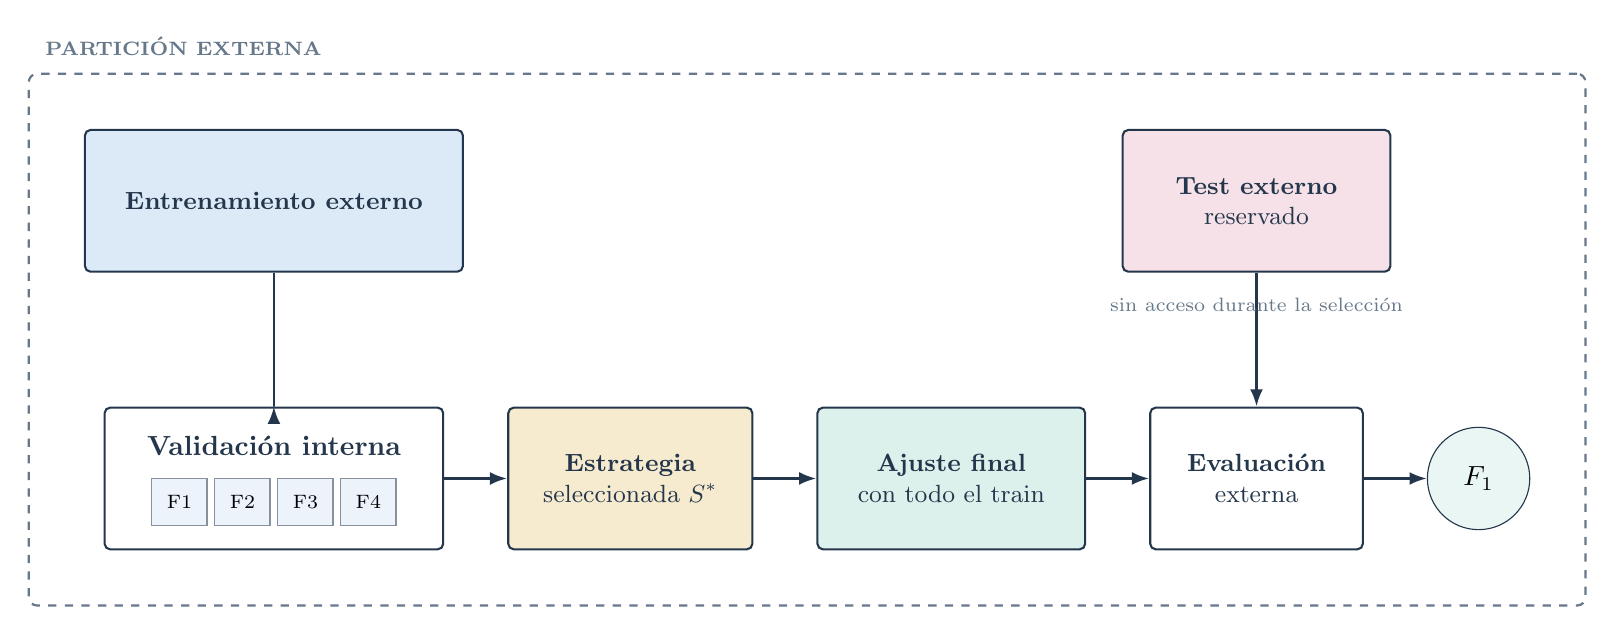
\begin{tikzpicture}[font=\small,node distance=8mm]
  \node[box,fill=blue,minimum width=48mm] (train) {\bfseries Entrenamiento externo};

  \node[box,fill=white,minimum width=43mm,below=17mm of train] (folds) {};
  \node[font=\bfseries,text=ink,anchor=north] at ([yshift=-2.5mm]folds.north) {Validación interna};
  \foreach \i in {1,...,4}{
    \node[draw=ink!55,fill=blue!55,minimum width=7mm,minimum height=6mm,font=\scriptsize]
      at ([xshift={-12mm+8mm*(\i-1)},yshift=-3mm]folds.center) {F\i};
  }
  \node[box,fill=amber,minimum width=31mm,right=of folds] (select) {\bfseries Estrategia\\seleccionada $S^*$};
  \node[box,fill=teal,minimum width=34mm,right=of select] (fit) {\bfseries Ajuste final\\con todo el train};
  \node[box,fill=white,minimum width=27mm,right=of fit] (eval) {\bfseries Evaluación\\externa};
  \node[draw=ink,circle,fill=teal!65,minimum size=13mm,right=of eval,font=\bfseries] (score) {$F_1$};
  \node[box,fill=rose,minimum width=34mm,above=17mm of eval] (test) {\bfseries Test externo\\reservado};

  \draw[flow] (train.south) |- (folds.north);
  \draw[flow] (folds) -- (select);
  \draw[flow] (select) -- (fit);
  \draw[flow] (fit) -- (eval);
  \draw[flow] (test) -- (eval);
  \draw[flow] (eval) -- (score);
  \node[small,below=2mm of test] {sin acceso durante la selección};

  \begin{scope}[on background layer]
    \node[draw=muted,dashed,rounded corners=3pt,line width=.8pt,fit=(train)(test)(folds)(score),inner sep=7mm] (outer) {};
  \end{scope}
  \node[font=\bfseries\scriptsize,text=muted,anchor=south west] at ([xshift=1mm,yshift=1mm]outer.north west) {PARTICIÓN EXTERNA};
\end{tikzpicture}
\end{document}
